In addition to the simulations above, we report results from a simple analysis of 
how male/female baby names evolve over time over the last century. 
The United States Social Security Administration provides a publicly available dataset listing the frequency of the 
top 1000 baby names in each state for the last 106 years.
We evaluate our model in this context to examine which ``sub-group'' of states tend to evolve (or change) in their
``name agreement" (or correlation) over time between boy names and girl names.
Here, rather than calculating a sample covariance
at each timepoint, we calculate a rank correlation matrix instead. 
For example, if two neighboring Gulf Coast states, say Georgia and Alabama, substantially 
agreed on both boys and girls names in the period following the second World War, but gradually this agreement 
declined over time for girls (but not boys), 
we expect that our scan statistics on graphs hypothesis test 
will segment out this differential signal (in slope trends) from the planar graph induced by the states sharing 
a border.
Shown in Figure \ref{fig:usmap} are the regions identified using our method, applied on only the rank correlations for the top 10 names for both genders per state per year. Each highlighted region indicates a sub-group
where their ``trends of correlation (or agreement/disagreement)'' in preferred baby names over the last century 
varies between boys and girls. 
%{\color{red} In Figure \ref{fig:babyEX} we show a snippet of the data from an identified subregion.}
%of states that have varying agreement and disagreement of boys and girls names over the last century.
For states not identified by our model (in gray), we can conclude that
the state-to-state name preference-interactions may have still 
evolved over time but we have insufficient statistical 
evidence to conclude that such trends (slopes) are different between boys and girls. 
%https://github.com/msbarry/babymap/
%may still have a strong trend in terms of how the
%state-to-state name preference-interactions 
%evolve over time but we have insufficient evidence to conclude that such trends are different between boys/girls. 
%tend to follow the trends of neighboring states very closely, regardless of sex. 

\begin{figure}
	\begin{center}
		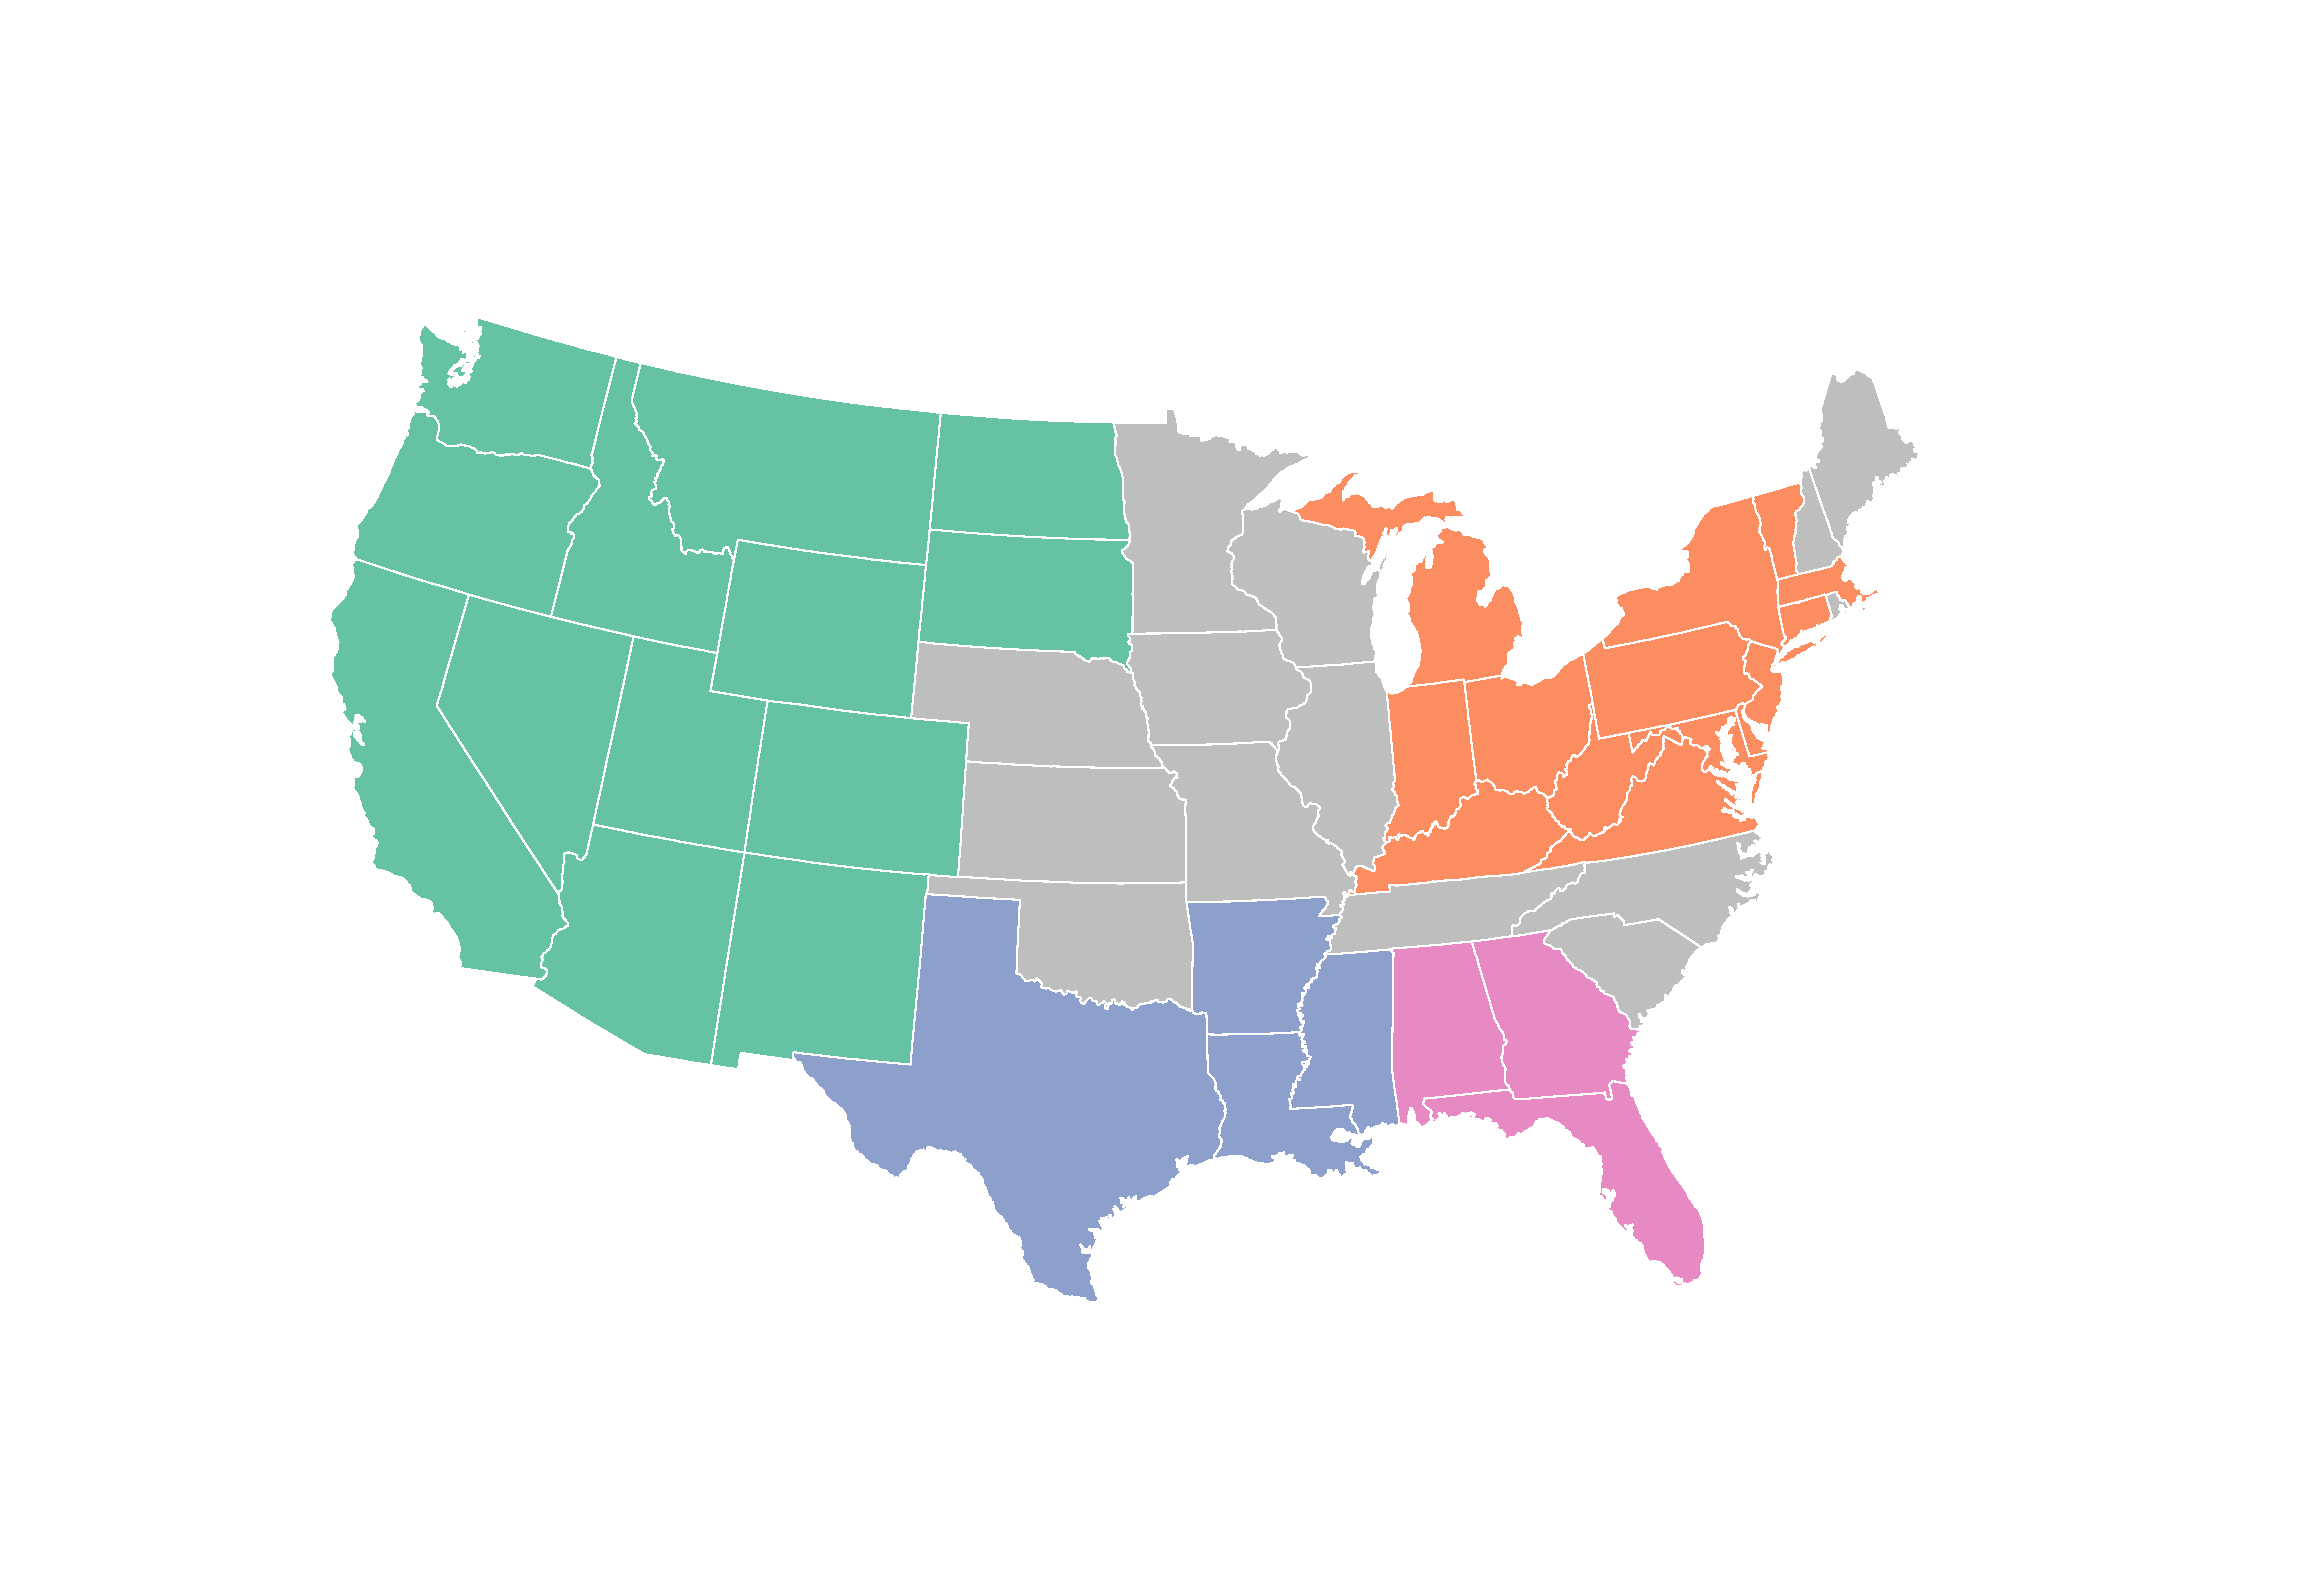
\includegraphics[,trim={5cm 5cm 5cm 5cm}, clip, width=0.7\textwidth]{3_covtraj/figs/babynames_res.eps}
		\caption[Covariance trajectory difference testing results on baby name frequency in the contiguous United States.]{\label{fig:usmap} Contiguous states identified as having significantly different time-varying co-occurrences between boys and girls baby names from 1910 to 2015. Best viewed in color.}
	\end{center}
\end{figure}